\chapter{Usage}

\section{Project Structure}

In order to use the project more efficiently I thought an explanation of the structure of the project would be a good place to start to further the understanding of the different elements of the project. \Cref{fig:struct} shows the structure.

\begin{figure}
    \centering
    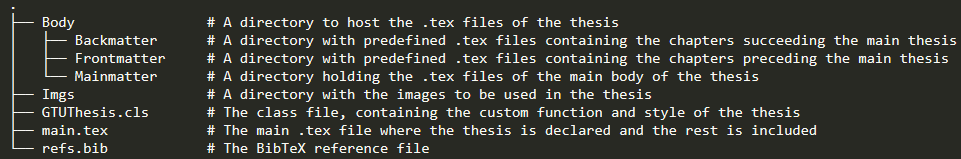
\includegraphics[width=\linewidth]{struct}
    \caption{The structure of the project, if too small please refer to the Github repo\cite{github}}
    \label{fig:struct}
\end{figure}


\section{Backmatter and Frontmatter}

As mentioned in the structure, these directories (\texttt{./Body/Backmatter} and \texttt{./Body/Frontmatter}) contain \texttt{.tex} files with the chapters preceding and succeeding the main body of the thesis, like abstract, list of acronyms, and appendices. The comments in the files themselves indicate where and what to write. Please don't edit the areas not meant to be edited.

\section{Mainmatter}\label{sec:mainmatter}

The \texttt{./Body/Mainmatter} directory is to house the \texttt{.tex} files of the main body of the thesis to be later included in the \texttt{./main.tex} (see \Cref{sec:maintex}). They can be named anything and organised within the directory in any way deemed fit. The example has two files (\texttt{C1.tex} and \texttt{C2.tex}) demonstrating a way of using the files, but it can be used in any other way, name or convention deemed appropriate by the user.

\section{Imgs and refs.bib}

As mentioned in the structure, \texttt{./Imgs} is a directory to house the images to be used in the figures of the thesis. The files in the directory could be further organised into subdirectories, but the file \texttt{./Imgs/gtu\_logo.jpg} to stay in its place.

As for \texttt{refs.bib}, this is a BibTeX file to be filled in with the references to be used for the thesis. (copied from the publisher or scholar.google.com)

\section{GTUThesis.cls}\label{sec:cls}

This is the file containing the custom functions and style of the GTU thesis. See \Cref{ch:class} for the documentation. \textbf{\textit{DO NOT}} modify this file unless you know what you're doing and sure about the changes you want to do.

\section{main.tex}\label{sec:maintex}

This is the main \texttt{.tex} file where the user firstly declares the document class as \texttt{GTUThesis} and then fills in the GTU-fields, followed by the used packages, and then starts the document environment, where they are expected to call the \texttt{GTUMakeFront} and \texttt{GTUMakeBack} functions respectively right after the start and before the end of the document environment. See \Cref{ch:class} for the documentation.

Between the \texttt{GTUMakeFront} and \texttt{GTUMakeBack} functions the user can include the files of the Main matter (recommended, see \Cref{sec:mainmatter}) using the include function as follows:

	\texttt{~~~~\textbackslash include\{./Body/Mainmatter/FILE.tex\}}

or write their thesis in the way they see fitting.

\section{Important Note}

\textbf{\textit{DO NOT}} delete, rename, or move the following files or directories because their paths are hard-coded:
\begin{itemize}
    \item \texttt{./Body}
    \item \texttt{./Body/Backmatter}
    \item \texttt{./Body/Backmatter/Appendices.tex}
    \item \texttt{./Body/Backmatter/CV.tex}
    \item \texttt{./Body/Frontmatter}
    \item \texttt{./Body/Frontmatter/Abstract.tex}
    \item \texttt{./Body/Frontmatter/Acknowledgement.tex}
    \item \texttt{./Body/Frontmatter/ListOfAcro.tex}
    \item \texttt{./Body/Frontmatter/Ozet.tex}
    \item \texttt{./Imgs}
    \item \texttt{./Imgs/gtu\_logo.jpg}
    \item \texttt{./GTUThesis.cls}
    \item \texttt{./refs.bib}
\end{itemize}